%%% Template originaly created by Karol Kozioł (mail@karol-koziol.net) and modified for ShareLaTeX use

\documentclass[a4paper,11pt]{article}

\usepackage[utf8]{inputenc}
\usepackage{kotex}

\renewcommand\familydefault{\sfdefault}

\usepackage{amsmath,amssymb,amsthm,textcomp}
\usepackage{enumerate}
\usepackage{minted}
\usepackage{xcolor}
\usepackage{hyperref}
\hypersetup{
    colorlinks=true,
    linkcolor=blue,
    filecolor=magenta,      
    urlcolor=cyan,
}
\urlstyle{same}
\usepackage{graphicx}

\usepackage{geometry}
\geometry{total={210mm,297mm},
left=25mm,right=25mm,%
bindingoffset=0mm, top=20mm,bottom=20mm}

\linespread{1.3}

\newcommand{\linia}{\rule{\linewidth}{0.5pt}}

% my own titles
\makeatletter
\renewcommand{\maketitle}{
\begin{center}
\vspace{2ex}
{\huge \textsc{\@title}}
\vspace{1ex}
\\
\linia\\
\@author \hfill \@date
\vspace{4ex}
\end{center}
}
\makeatother
%%%

% custom footers and headers
\usepackage{fancyhdr}
\pagestyle{fancy}
\lhead{}
\chead{}
\rhead{}
\lfoot{Homework \#2}
\cfoot{}
\rfoot{Page \thepage}
\renewcommand{\headrulewidth}{0pt}
\renewcommand{\footrulewidth}{0pt}
%

\renewcommand\listoflistingscaption{List of source codes}

\begin{document}

\title{Operating Systems Homework \#2}

\author{김현준 (2012003954), 한양대학교}

\date{2015-05-07}

\maketitle

\section*{The Dining Philosophers Problem}

\subsection*{Comments on this homework:}
    유명한 철학자 문제를 직접 구현해볼 수 있어 즐거운 과제였습니다.
    처음에는 강의 시간에 교수님께서 예로 들어주신 것처럼 짝수번째 철학자와 홀수번째 철학자가 서로 다른 방향의 젓가락을 먼저 차지하는 전략으로 구현했고, 이후에는 최대 {{N - 1}}명의 철학자만 동시에 젓가락을 집으려고 시도할 수 있도록 제한하는 방법으로 다시 구현하였습니다(\url{https://github.com/yoloseem/os-homeworks/commit/682dbaf643b1028d4823e4239e0d96e48c8c21d8}). 이와 같이 여러 방법을 시도해보면서 문제를 해결하는데에는 다양한 방법이 존재할 수 있음을 다시금 경험할 수 있었고, 그와 동시에 여러 해결책을 생각해내기 위해서는 기반 지식과 경험 역시 탄탄해야하겠다고 생각했습니다. 예컨대, 최대 {{N - 1}}명을 허용하는데에 Semaphore를 사용하는 방법은, 단순히 단일 트랜잭션에 대한 Lock으로만, 즉 Binary Semaphore로서만 이해하고 있던 저로서는 이번 과제를 하면서 제대로 알 수 있게된 부분입니다.
    
    과제 내용과 별개로 기억에 남는 것은, 과제 구현을 시작할 때부터 {{Makefile}}을 만들어두었더니 매 코드 변경시마다 컴파일 및 실행을 간편하게 할 수 있어서 좋았습니다.

\subsection*{References:}
\begin{enumerate}
\item
    Full HW description:

        \url{https://github.com/yoloseem/os-homeworks/blob/master/hw2/README.md}

\item
    Raw source codes:

        \url{https://github.com/yoloseem/os-homeworks/tree/master/hw2}

\item
    Commit history:

        \url{https://github.com/yoloseem/os-homeworks/commits/master}
\end{enumerate}

\subsection*{Screenshot:}
    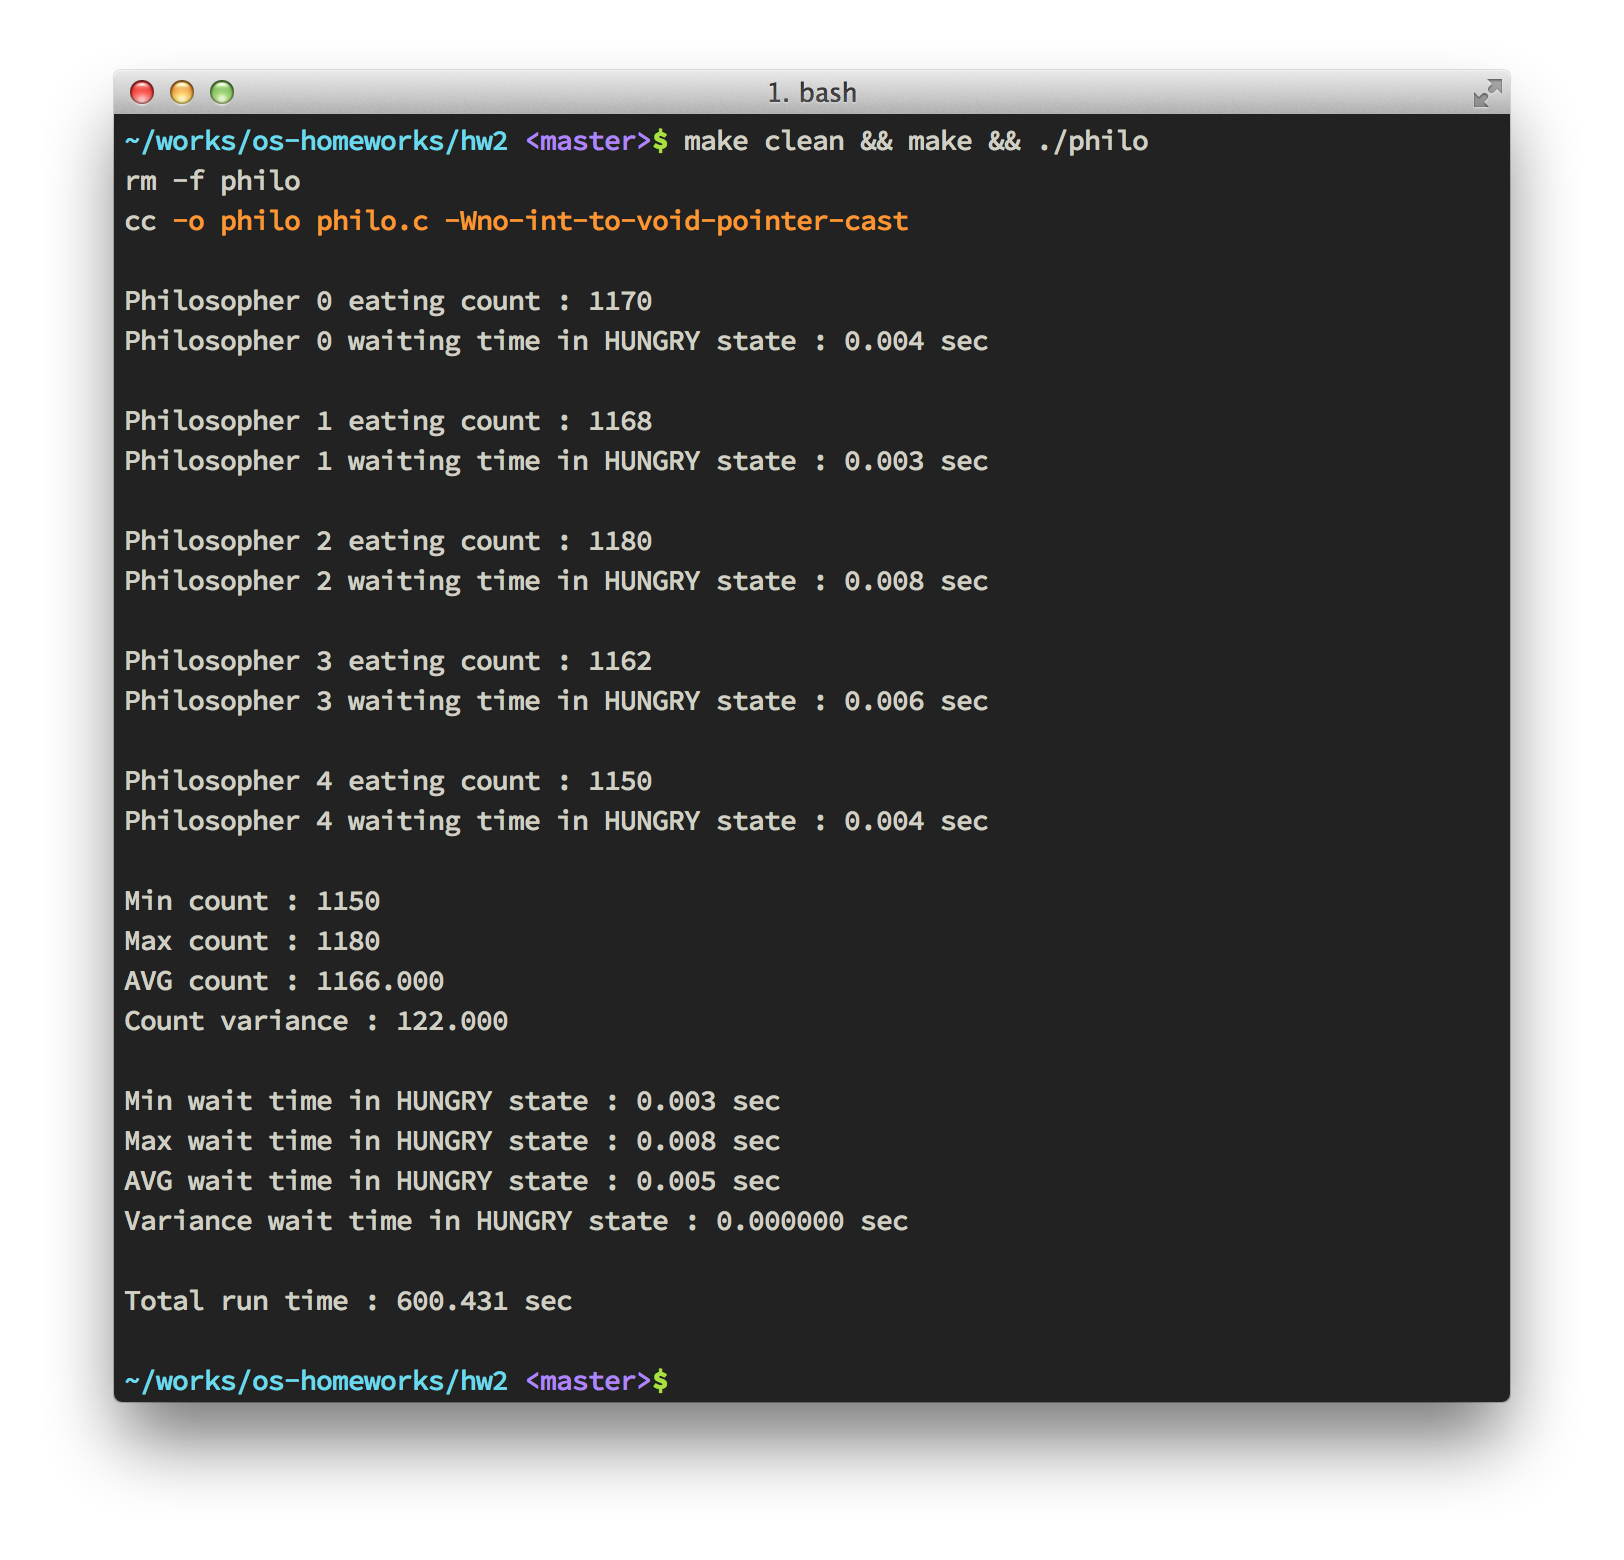
\includegraphics[width=\textwidth]{screenshot.png}

\subsection*{Source codes:}

\subsubsection*{Makefile}
\inputminted[fontsize=\footnotesize,linenos]{basemake}{Makefile}

\subsubsection*{philo.c (Main source code)}
\inputminted[fontsize=\footnotesize,linenos]{c}{philo.c}

\end{document}
